\documentclass{myreport}

\usepackage{tabularray}
\usepackage{float}
\usepackage{graphicx}
\usepackage{codehigh}
\usepackage[normalem]{ulem}
\usepackage{longtable}

% References
\bibliographystyle{copernicus.bst}

\begin{document}
\pagestyle{headings}

% Change figure (table, section) numbering (e.g., from 'Figure 1' to 'Figure S1')
\renewcommand{\thefigure}{S\arabic{figure}}
\renewcommand{\thetable}{S\arabic{table}}
\renewcommand{\thesection}{S\arabic{section}}
\renewcommand{\theequation}{S\arabic{equation}}

% Document must include
% ---------------------
%

%% Title
\title{SUPPLEMENTARY INFORMATION:\\
Global forest thickening}
\author{Marqués et al.}

\maketitle

\tableofcontents

%%%%%%%%%%%%%%%%%%%%%%%%%%%%%%%
\section{Data}
%%%%%%%%%%%%%%%%%%%%%%%%%%%%%%%

Quadratic mean diameter (QMD) was derived at the stand level using a harmonised approach across datasets that differed in their level of aggregation.

When individual tree measurements were available, stand basal area (BA) and stand density ($N$) were first calculated by aggregating tree-level data by plot and census year. Basal area was computed as the sum of individual tree basal area and expressed per unit ground area, while stand density was calculated as the number of trees per unit area. When stand-level data were provided directly, reported values of basal area and stand density were used without further aggregation.

BA (ha$^{-1}$) is related to tree diameters as

\begin{equation}
\mathrm{BA} = \frac{\pi}{4} \sum_{i=1}^{N} d_i^2,
\label{eq:ba}
\end{equation}

where $d_i$ is the diameter at breast height of an individual tree, and $N$ is the total number of trees in a given reference area, i.e., the stand density (trees ha$^{-1}$). The quadratic mean diameter (QMD) is defined as

\begin{equation}
\mathrm{QMD} = \sqrt{\frac{1}{N} \sum_{i=1}^{N} d_i^2}.
\label{eq:qmd}
\end{equation}

Substituting the definition of basal area (Eq. \ref{eq:ba}) into Eq. \ref{eq:qmd} leads to

\begin{equation}
\mathrm{QMD} = \sqrt{\frac{4\,\mathrm{BA}}{\pi N}}.
\label{eq:qmd2}
\end{equation}

In practice, QMD was calculated from stand basal area ($\mathrm{m^2\,ha^{-1}}$) and stand density (trees ha$^{-1}$). All variables were harmonised to SI units prior to analysis to ensure comparability across inventories differing in measurement units and sampling design.


\begin{table}
  % \label{tab:datasets}
\centering
\fontsize{8}{10}\selectfont
\begin{tabular}{llp{4cm}p{4cm}p{4cm}}
  \toprule
Dataset & \textit{N} & Description & Filter & Reference \\
    \midrule
  nfi\_spain & 27642 & Spanish National Forest Inventory & No management intervention observed during monitoring & Restricted data (not publicly available) \\
  nfi\_norway & 25156 & Norwegian National Forest Inventory & No management intervention observed during monitoring & Restricted data (not publicly available) \\
  nfi\_sweeden & 15954 & Swedish National Forest Inventory & No management intervention observed during monitoring & Restricted data (not publicly available) \\
  bnp & 9423 & Berchtesgaden National Park & Forest reserves & Restricted data (not publicly available) \\
  fia\_us & 7022 & Forest Inventory and Analysis, US & Forest reserves & Doser JW, Stanke H, Finley AO (2025). rFIA: Estimation of Forest Variables using the FIA Database. R package version 1.1.0, https://CRAN.R-project.org/package=rFIA \\
  aus\_plots & 6259 & Sustainable Timber Tasmania, Forestry Corporation of NSW, Queensland, Victoria and Australia's Terrestrial Ecosystem Research Network & No management intervention observed during monitoring & Restricted data (not publicly available) \\
  luquillo & 1993 & Luquillo & No management intervention observed during monitoring & https://forestgeo.si.edu \\
  nfi\_switzerland & 1972 & Swiss National Forest Inventory & No management intervention observed during the last 70 years & Restricted data (not publicly available) \\
  scbi & 1572 & Smithsonian Conservation Biology Institute & No management intervention observed during monitoring & https://forestgeo.si.edu \\
  wuls & 1416 & Białowieża National Park & Forest reserves & Restricted data (not publicly available) \\
  wytham & 1200 & Wytham Woods & No management intervention observed during monitoring & https://forestgeo.si.edu \\
  serc & 1026 & Smithsonian Environmental Research Center & No management intervention observed during monitoring & https://forestgeo.si.edu \\
  pasoh & 1007 & Pasoh & No management intervention observed during monitoring & https://forestgeo.si.edu \\
  df\_rainfor & 988 & Amazon Forest Inventory Network (RAINFOR) & No management intervention ocurred & Esquivel-Muelbert, A., Banbury Morgan, R., Brienen, R. et al. Increasing tree size across Amazonia. Nat. Plants 11, 2016–2025 (2025). https://doi.org/10.1038/s41477-025-02097-4 \\
  nfr\_swi & 729 & Swiss Natural Forest Reserves & Forest reserves & Restricted data (not publicly available) \\
  forst & 537 & Forest Research Institute Baden-Württemberg & Forest reserves & Restricted data (not publicly available) \\
  palanam & 484 & No management intervention observed during monitoring & https://forestgeo.si.edu \\
  unito & 311 & University of Turin  & Forest reserves & Restricted data (not publicly available) \\
  uholka & 200 & Uholka-Shyrokyi Luh & Forest reserves & Restricted data (not publicly available) \\
  df\_forestplots & 149 & Forest Inventory Network & No management intervention ocurred & Restricted data (not publicly available) \\
  mudumalai & 126 & Mudumalai & No management intervention observed during monitoring & Restricted data (not publicly available) \\
  lwf\_tree & 114 & Bavarian Institute of Forestry & Forest reserves & Restricted data (not publicly available) \\
  nwfva\_tree & 84 &  Northwest German Forest Research Institute (NW-FVA) & Forest reserves & Restricted data (not publicly available) \\
  \bottomrule
  \end{tabular}
\caption{Constituent forest dataset sizes and descriptions.}
\end{table}

\begin{table}
  % \label{tab:datasets}
\centering
\fontsize{8}{10}\selectfont
\begin{tabular}{llp{4cm}p{4cm}p{4cm}}
  \toprule
Dataset & N & Description & Filter & Reference \\
    \midrule
  incds &  75 & National Institute for Research-Development in Forestry ‘‘Marin Drăcea’’ Department of Forest & Forest reserves & Restricted data (not publicly available) \\
  tuzvo\_tree &  63 & Technical University in Zvolen & Forest reserves & Restricted data (not publicly available) \\
  iberbas &  57 & Institute of Biodiversity and Ecosystem Research, Bulgarian Academy of Sciences & Forest reserves & Restricted data (not publicly available) \\
  efm\_swi &  51 & Experiemental Forest Management plots & No management intervention observed during monitoring & Restricted data (not publicly available) \\
  france & 47 & French plots & No management intervention observed during monitoring & Restricted data (not publicly available) \\
  greece\_stand &  40 & Greek plots & No management intervention observed during monitoring & Restricted data (not publicly available) \\
  czu &  24 & Czech University of Life Sciences Prague & Forest reserves & Restricted data (not publicly available) \\
  ul\_tree &  23 & University of Ljubljana, Slovenia & Forest reserves & Restricted data (not publicly available) \\
  urk &  12 & Roztocze National Park, Poland & Forest reserves & Restricted data (not publicly available) \\
  nbw & 7 & NPV-BW & Forest reserves & Restricted data (not publicly available) \\
  \bottomrule
  \end{tabular}
\caption{Constituent forest dataset sizes and descriptions.}
\end{table}

\clearpage

\begin{figure}
\centering
\includegraphics[width=\textwidth]{../figures/gg_sitepoints.pdf}
\caption{Distribution of forest plots (red circles) and forest biomes.}
\end{figure}

\begin{figure}
\centering
\includegraphics[width=0.9\textwidth]{../figures/distribution_length.pdf}
\caption{Distribution of the total length of the time series per forest plot, separated by biomes. The total length corresponds to the difference in the observation year of the first and last available forest inventory for each plot.}
\end{figure}

\begin{figure}
\centering
\includegraphics[width=0.9\textwidth]{../figures/fig_hist_year.pdf}
\caption{Distribution of forest census data over time, grouped by biome (a-f). Dataset names are explained in Tab. S1.}
\end{figure}

\clearpage

%%%%%%%%%%%%%%%%%%%%%%%%%%%%%%%
\section{Self-thinning trends}
%%%%%%%%%%%%%%%%%%%%%%%%%%%%%%%

\begin{figure}
\centering
\includegraphics[width=\textwidth]{../figures/stl_longplots.pdf}
\caption{Self-thinning relation across biomes with example long-term forest monitoring plots highlighted.}
\end{figure}

\begin{figure}
\centering
\includegraphics[width=\textwidth]{../figures/slope_distribution.pdf}
\caption{Distributions of model slope estimates (logQMD) across biomes.}
\end{figure}

\begin{figure}
\centering
\includegraphics[width=\textwidth]{../figures/fig1_lqmm_onlydots.pdf}
\caption{Effect size of 'year' within bins of quadratic mean diameter for individual biomes (a: Tropical and Subtropical Moist Broadleaf Forests, b: Tropical and Subtropical Dry Broadleaf Forests, c: Temperate Broadleaf and Mixed Forests, d: Temperate Conifer Forests Forest, e: Boreal Forests/Taiga, f: Mediterranean Forests). Grey points represent the same derived from data before the filtering of disturbance-affected plots were removed. Error bars indicate 95\% confidence intervals for the coefficient.}
\end{figure}

\begin{figure}
\centering
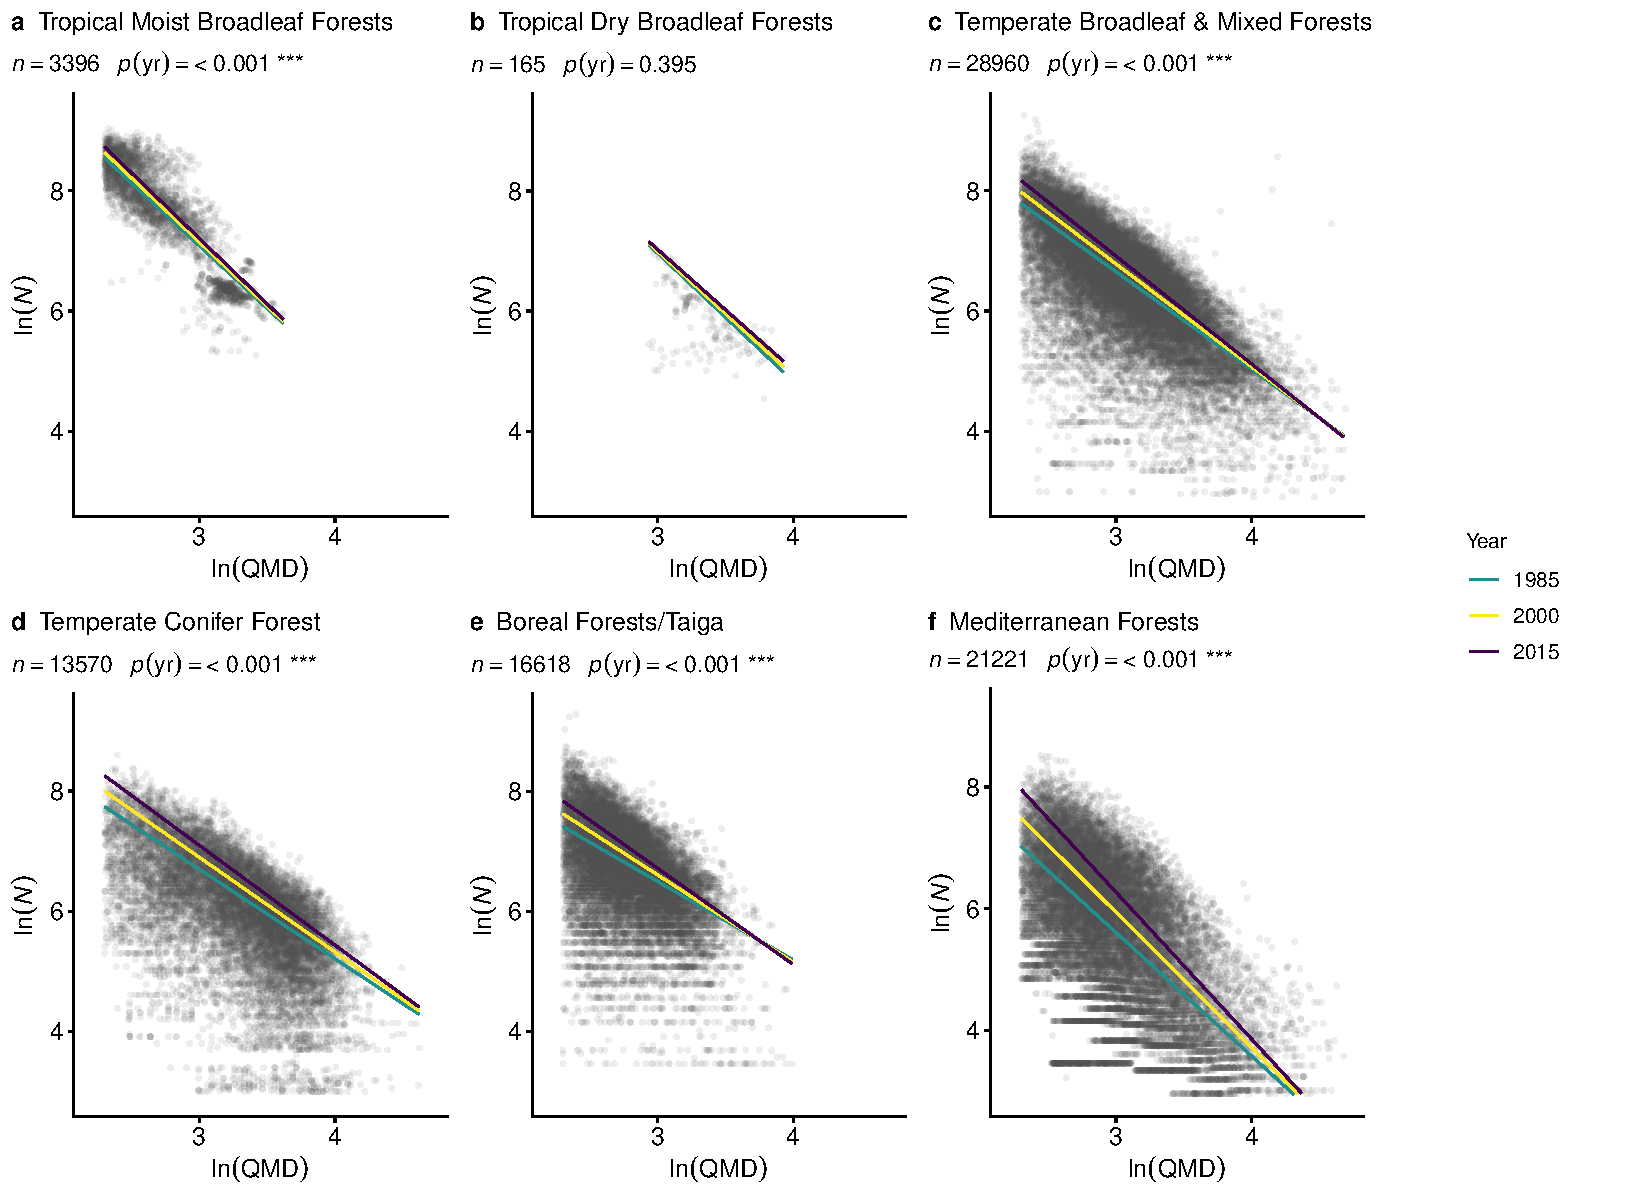
\includegraphics[width=\textwidth]{../figures/fig1_lqmm_int_onlystl.pdf}
\caption{Forest self-thinning relationship and its temporal change by biome, considering temporal changes in the self-thinning slope (interaction between `year' and `logQMD'). Panels a-f show stand density (N, trees ha$^\text{ha}$, log-scale) as a function of quadratic mean diameter (QMD, cm, log-scale) and calendar year over the study period, across six forest biomes. Grey points represent data from selected unmanaged and undisturbed forest plots. Coloured lines represent the fitted relationship between year and stand density at the 0.9 quantile. The number of observations for each biome (n) and the significance level (p-value, asymptotic Wald-type tests) for the predictor year (p(yr)) are given as subtitle annotations within each panel.}
\end{figure}

% XXX todo: visualise evolution of individual forest plots for a small subset of plots, selected based on length of available time series.

% Example for how to include a table, generated externally
% Uses library xtable.
% Function create_table_latex() is included also in this repo.
% R code that was used to create this example table:
% df_experiments_co2_asat <- df5 |>
%   filter(myvar == "asat") |>
%   select(exp, myvar) |>
%   left_join(
%     df |>
%       select(exp, myvar = response, citation),
%     by = join_by(exp, myvar)
%   ) |>
%   select(exp, citation) |>
%   distinct() |>
%
%   # format for processing with latex
%   mutate(citation = paste0('\\', "cite{", citation, "}")) |>
%   group_by(exp) |>
%   summarise(
%     citation = paste0(unique(citation), collapse = ", ")
%   ) |>
%   rename(
%     Experiment = exp,
%     Reference = citation
%   )

% % latex table generated in R 4.5.0 by xtable 1.8-4 package
% Thu Nov 27 09:47:09 2025
\begin{table}[ht]
\centering
\begin{tabular}{lll}
  \hline
Biome & Mean & SD \\ 
  \hline
Boreal Forests/Taiga & 0.30 & 0.06 \\ 
  Mediterranean Forests & 2.35 & 0.06 \\ 
  Temperate Broadleaf \& Mixed Forests & 0.91 & 0.03 \\ 
  Temperate Conifer Forests & 1.18 & 0.06 \\ 
  Tropical \& Subtropical Moist Broadleaf Forests & 0.16 & 0.07 \\ 
  Tropical Dry Broadleaf Forests & -0.38 & 0.46 \\ 
  \end{tabular}
\caption{Percentage change of forest stand density.} 
\end{table}


\begin{table}
\centering
\begin{tabular}{lll}
  \toprule
Biome & Mean & SE \\
  \midrule
  Boreal Forests/Taiga & 0.30 & 0.06 \\
  Mediterranean Forests & 2.35 & 0.06 \\
  Temperate Broadleaf \& Mixed Forests & 0.91 & 0.03 \\
  Temperate Conifer Forests & 1.18 & 0.06 \\
  Tropical \& Subtropical Moist Broadleaf Forests & 0.16 & 0.07 \\
  Tropical Dry Broadleaf Forests & -0.38 & 0.46 \\
  \bottomrule
  \end{tabular}
\caption{Mean estimate and standard error (SE) of percentage change (\%/yr) of forest stand density (number of trees per ha) by biome, determined from quantile regressions on bootstrapped data samples.}
\end{table}


\begin{figure}
\centering
\includegraphics[width=\textwidth]{../figures/hist_percent_change.pdf}
\caption{Distribution of percentage change (\%/yr) in stand density (number of trees per ha) by biome.}
\end{figure}


\begin{figure}
\centering
\includegraphics[width=\textwidth]{../figures/fdisturbed.pdf}
\caption{Trends in the fraction of disturbed forest plots, by biome. Fraction values are logit-transformed. The corresponding un-transformed values are indicated by the right y-axis in each plot. No regression fit is shown for tropical dry broadleaf forests (b) as only two points are available with non-zero values for the disturbed fraction.}
\end{figure}

\clearpage

%%%%%%%%%%%%%%%%%%%%%%%%%%%%%%%
\section{Environmental drivers}
%%%%%%%%%%%%%%%%%%%%%%%%%%%%%%%

\begin{table}
\centering
\scriptsize
\begin{talltblr}[         %% tabularray outer open
caption={Regression Results},
]                     %% tabularray outer close
{                     %% tabularray inner open
colspec={Q[]Q[]Q[]Q[]Q[]},
column{2,3,4,5}={}{halign=c,},
column{1}={}{halign=l,},
hline{31}={1,2,3,4,5}{solid, black, 0.05em},
}                     %% tabularray inner close
\toprule
& Complete & No PBR & No PBR, ORGC & No PBR, C:N \\ \midrule %% TinyTableHeader
scale(logQMD) & -0.861*** & -0.862*** & -0.862*** & -0.864*** \\
& [-0.865, -0.856] & [-0.867, -0.858] & [-0.867, -0.857] & [-0.869, -0.859] \\
scale(year) & 0.129*** & 0.130*** & 0.130*** & 0.132*** \\
& [0.126, 0.132] & [0.127, 0.133] & [0.128, 0.133] & [0.129, 0.135] \\
scale(tavg) & -0.033* & -0.026+ & -0.007 & -0.018 \\
& [-0.062, -0.003] & [-0.055, 0.002] & [-0.034, 0.020] & [-0.046, 0.011] \\
scale(ai) & 0.086*** & 0.095*** & 0.097*** & 0.087*** \\
& [0.066, 0.105] & [0.077, 0.114] & [0.079, 0.115] & [0.070, 0.105] \\
scale(ndep) & 0.153*** & 0.140*** & 0.146*** & 0.131*** \\
& [0.133, 0.174] & [0.120, 0.159] & [0.127, 0.166] & [0.112, 0.151] \\
scale(ORGC) & -0.039** & -0.048*** &  & -0.001 \\
& [-0.064, -0.014] & [-0.073, -0.024] &  & [-0.019, 0.017] \\
scale(PBR) & 0.004 &  &  &  \\
& [-0.012, 0.021] &  &  &  \\
scale(CNrt) & 0.057*** & 0.060*** & 0.031*** &  \\
& [0.035, 0.079] & [0.039, 0.081] & [0.015, 0.047] &  \\
scale(year) × scale(tavg) & 0.006** & 0.009*** & 0.013*** & 0.006** \\
& [0.002, 0.011] & [0.005, 0.013] & [0.009, 0.017] & [0.002, 0.010] \\
scale(year) × scale(ai) & -0.022*** & -0.018*** & -0.018*** & -0.017*** \\
& [-0.025, -0.019] & [-0.021, -0.015] & [-0.020, -0.015] & [-0.019, -0.014] \\
scale(year) × scale(ndep) & -0.016*** & -0.015*** & -0.015*** & -0.011*** \\
& [-0.019, -0.013] & [-0.018, -0.012] & [-0.018, -0.012] & [-0.013, -0.008] \\
scale(year) × scale(ORGC) & -0.012*** & -0.011*** &  & -0.028*** \\
& [-0.017, -0.008] & [-0.015, -0.007] &  & [-0.032, -0.025] \\
scale(year) × scale(PBR) & 0.006*** &  &  &  \\
& [0.002, 0.009] &  &  &  \\
scale(year) × scale(CNrt) & -0.021*** & -0.023*** & -0.028*** &  \\
& [-0.025, -0.017] & [-0.026, -0.019] & [-0.031, -0.025] &  \\
SD (Observations) & 0.176 & 0.178 & 0.178 & 0.178 \\
Num.Obs. & 36133 & 37652 & 37652 & 37652 \\
R2 Marg. & 0.521 & 0.530 & 0.531 & 0.527 \\
R2 Cond. & 0.980 & 0.980 & 0.980 & 0.980 \\
AIC & 17693.1 & 19142.8 & 19162.9 & 19315.9 \\
BIC & 17846.0 & 19279.3 & 19282.4 & 19435.4 \\
ICC & 1.0 & 1.0 & 1.0 & 1.0 \\
RMSE & 0.15 & 0.15 & 0.15 & 0.15 \\
\bottomrule
\end{talltblr}
\end{table}


\begin{table}
\centering
\scriptsize
\begin{talltblr}[         %% tabularray outer open
caption={Regression Results},
]                     %% tabularray outer close
{                     %% tabularray inner open
colspec={Q[]Q[]},
column{2}={}{halign=c,},
column{1}={}{halign=l,},
hline{43}={1,2}{solid, black, 0.05em},
}                     %% tabularray inner close
\toprule
& Complete interactions \\ \midrule %% TinyTableHeader
scale(logQMD) & -0.830*** \\
& [-0.835, -0.826] \\
scale(year) & 0.120*** \\
& [0.117, 0.123] \\
scale(tavg) & -0.014 \\
& [-0.043, 0.016] \\
scale(ai) & 0.101*** \\
& [0.082, 0.120] \\
scale(ndep) & 0.129*** \\
& [0.109, 0.150] \\
scale(ORGC) & -0.024+ \\
& [-0.048, 0.001] \\
scale(PBR) & -0.005 \\
& [-0.021, 0.011] \\
scale(CNrt) & 0.062*** \\
& [0.040, 0.084] \\
scale(year) × scale(tavg) & -0.006* \\
& [-0.010, -0.001] \\
scale(year) × scale(ai) & -0.033*** \\
& [-0.036, -0.030] \\
scale(year) × scale(ndep) & -0.012*** \\
& [-0.015, -0.009] \\
scale(year) × scale(ORGC) & -0.011*** \\
& [-0.015, -0.006] \\
scale(year) × scale(PBR) & -0.001 \\
& [-0.005, 0.002] \\
scale(year) × scale(CNrt) & -0.029*** \\
& [-0.033, -0.026] \\
scale(logQMD) × scale(tavg) & 0.020*** \\
& [0.012, 0.027] \\
scale(logQMD) × scale(ai) & 0.102*** \\
& [0.097, 0.108] \\
scale(logQMD) × scale(ndep) & -0.021*** \\
& [-0.026, -0.016] \\
scale(logQMD) × scale(ORGC) & -0.009* \\
& [-0.017, -0.000] \\
scale(logQMD) × scale(PBR) & 0.017*** \\
& [0.012, 0.022] \\
scale(logQMD) × scale(CNrt) & 0.047*** \\
& [0.040, 0.053] \\
SD (Observations) & 0.171 \\
Num.Obs. & 36133 \\
R2 Marg. & 0.515 \\
R2 Cond. & 0.980 \\
AIC & 15842.4 \\
BIC & 16046.3 \\
ICC & 1.0 \\
RMSE & 0.14 \\
\bottomrule
\end{talltblr}
\end{table}


% \begin{table}
\centering
\begin{talltblr}[         %% tabularray outer open
caption={Regression Results},
]                     %% tabularray outer close
{                     %% tabularray inner open
colspec={Q[]Q[]Q[]Q[]Q[]},
column{2,3,4,5}={}{halign=c,},
column{1}={}{halign=l,},
hline{31}={1,2,3,4,5}{solid, black, 0.05em},
}                     %% tabularray inner close
\toprule
& Complete & No PBR & No PBR, ORGC & No PBR, C:N \\ \midrule %% TinyTableHeader
scale(logQMD) & -0.646*** & -0.645*** & -0.645*** & -0.645*** \\
& (0.002) & (0.002) & (0.002) & (0.002) \\
scale(year) & 0.064*** & 0.064*** & 0.065*** & 0.065*** \\
& (0.001) & (0.001) & (0.001) & (0.001) \\
scale(tavg) & 0.025*** & 0.020** & 0.018* & 0.022** \\
& (0.007) & (0.007) & (0.007) & (0.007) \\
scale(ai) & 0.060*** & 0.059*** & 0.059*** & 0.059*** \\
& (0.004) & (0.004) & (0.004) & (0.004) \\
scale(ndep) & 0.042*** & 0.043*** & 0.043*** & 0.042*** \\
& (0.004) & (0.004) & (0.004) & (0.004) \\
scale(ORGC) & 0.007 & 0.005 &  & 0.006 \\
& (0.005) & (0.005) &  & (0.004) \\
scale(PBR) & 0.004 &  &  &  \\
& (0.003) &  &  &  \\
scale(CNrt) & -0.001 & -0.001 & 0.002 &  \\
& (0.004) & (0.004) & (0.003) &  \\
scale(year) × scale(tavg) & -0.007*** & -0.007*** & -0.004* & -0.007*** \\
& (0.002) & (0.001) & (0.001) & (0.001) \\
scale(year) × scale(ai) & -0.009*** & -0.008*** & -0.008*** & -0.007*** \\
& (0.001) & (0.001) & (0.001) & (0.001) \\
scale(year) × scale(ndep) & -0.005*** & -0.006*** & -0.006*** & -0.002 \\
& (0.001) & (0.001) & (0.001) & (0.001) \\
scale(year) × scale(ORGC) & -0.012*** & -0.011*** &  & -0.026*** \\
& (0.002) & (0.002) &  & (0.001) \\
scale(year) × scale(PBR) & 0.003+ &  &  &  \\
& (0.001) &  &  &  \\
scale(year) × scale(CNrt) & -0.019*** & -0.021*** & -0.027*** &  \\
& (0.002) & (0.001) & (0.001) &  \\
SD (Observations) & 0.109 & 0.110 & 0.110 & 0.111 \\
Num.Obs. & 22566 & 23570 & 23570 & 23570 \\
R2 Marg. & 0.728 & 0.712 & 0.710 & 0.711 \\
R2 Cond. & 0.979 & 0.980 & 0.979 & 0.979 \\
AIC & -13634.4 & -13910.0 & -13889.1 & -13732.0 \\
BIC & -13490.0 & -13780.9 & -13776.1 & -13619.0 \\
ICC & 0.9 & 0.9 & 0.9 & 0.9 \\
RMSE & 0.09 & 0.09 & 0.09 & 0.09 \\
\bottomrule
\end{talltblr}
\end{table}


\clearpage

% \begin{figure}
% \centering
% \includegraphics[width=0.8\textwidth]{../figures/coefs_env_quantilefilter.pdf}
% \caption{Coefficients of fixed effects of environmental factors on the self-thinning relationship. Data was filtered to retain observations from plots subject to dominant self-thinning dynamics based on quantiles within QMD bins, following Marqués et al. xxx}
% \end{figure}

% \begin{figure}
% \centering
% \includegraphics[width=0.8\textwidth]{../figures/coefs_env_slopefilter.pdf}
% \caption{Coefficients of fixed effects of environmental factors on the self-thinning relationship. Data was filtered to retain observations from plots subject to dominant self-thinning dynamics based on slopes.}
% \end{figure}
%
% \clearpage

%%%%%%%%%%%%%%%%%%%%%%%%%%%%%%%
\section{Global C sink}
%%%%%%%%%%%%%%%%%%%%%%%%%%%%%%%

\begin{figure}[ht!]
\centering
\includegraphics[width=\textwidth]{../figures/gg_map_sink_perforestarea_combined.pdf}
\caption{(a) C sink in aboveground biomass due to temporal changes in the self-thinning relationship. (b) Standard deviation of estimates across bootstraps. Values are expressed per unit forest area (MgC ha$^{-2}$ yr$^{-1}$).}
\end{figure}



%%%%%%%%%%%%%%%%%%%%%%%%%%%%%%%%%%%%%%%%%%%%%%%%%%%%%%%%%%%%%%%%%%%%%%%%%%%
\clearpage
\bibliography{references_global_forest_thickening.bib}


\end{document}
